\newpage

\section{Вычислительный эксперимент}

Для анализа моделей, полученных путем дистилляции модели учителя в модель ученика, проводится вычислительный эксперимент для задачи классификации.\\
Эксперимент проводится для выборки FashionMNIST~\cite{FMNIST} - набора изображений предметов одежды. В качестве моделей учителя $\textbf{f}$ и ученика $\textbf{g}$ рассматриваются четырёхслойная и однослойная нейронные сети соответсвенно. Для решения оптимизационной задачи используется Adam, функция активации - ReLu.\\
Выборка разделяется на 3 части: две для обучения многоресурного и малоресурсного доменов, а также тестовая часть выборки. Многоресурсная часть содержит 59000 объектов, малоресурсная часть содержит 1000 объектов, а тестовая часть содержит 10000 объектов.
\newpage
\subsection{Анализ дистилляции Хинтона}

\textbf{Обучение на обоих доменах}\\
На рис.1а показан график зависимости метрики accuracy на тестовой выборке между истинными метками объектов и вероятностями, предсказанными моделью ученика.\\
На рис.1б показан график зависимости кросс-энтропии на тестовой выборке между истинными метками объектов и вероятностями, предсказанными моделью ученика.\\
На графиках видно, что модель, использующая метки учителя, показывает лучшее значение accuracy, при этом наблюдается незначительное повышение ошибки.
\begin{figure}[h!t]\center
\subfloat[]
{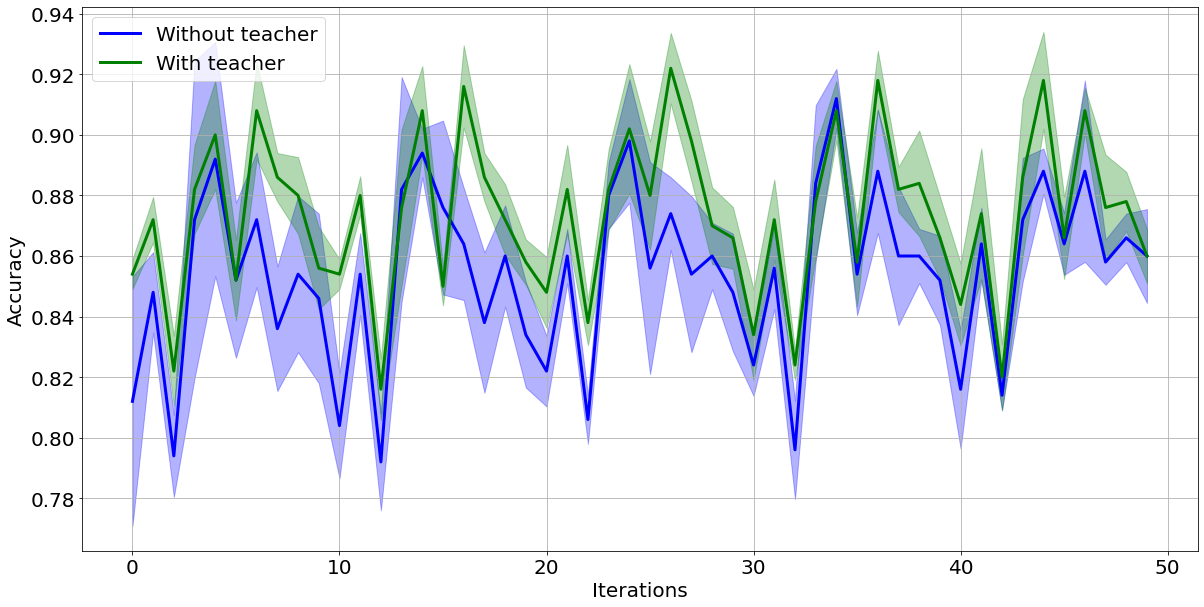
\includegraphics[width=0.5\textwidth]{results/accuracy}}
\subfloat[]
{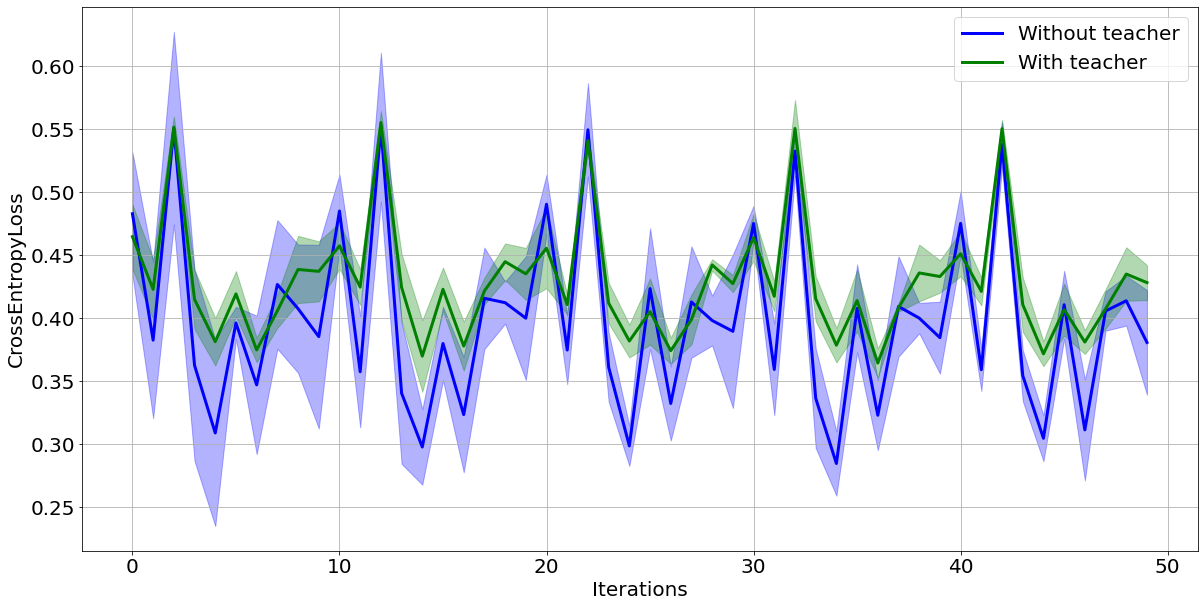
\includegraphics[width=0.5\textwidth]{results/loss}}\\
\caption{Качество аппроксимации на тестовой выборке a) accuracy; b) CrossEntropyLoss между истинными и предсказанными учеником метками}
\end{figure}

\newpage
\textbf{Обучение на многоресурсном домене}
На рис.1а показан график зависимости метрики accuracy на тестовой выборке между истинными метками объектов и вероятностями, предсказанными моделью ученика.\\
На рис.1б показан график зависимости кросс-энтропии на тестовой выборке между истинными метками объектов и вероятностями, предсказанными моделью ученика.\\
На графиках видно, что модель, использующая метки учителя, показывает лучшее значение accuracy, при этом наблюдается незначительное повышение ошибки.
\begin{figure}[h!t]\center
\subfloat[]
{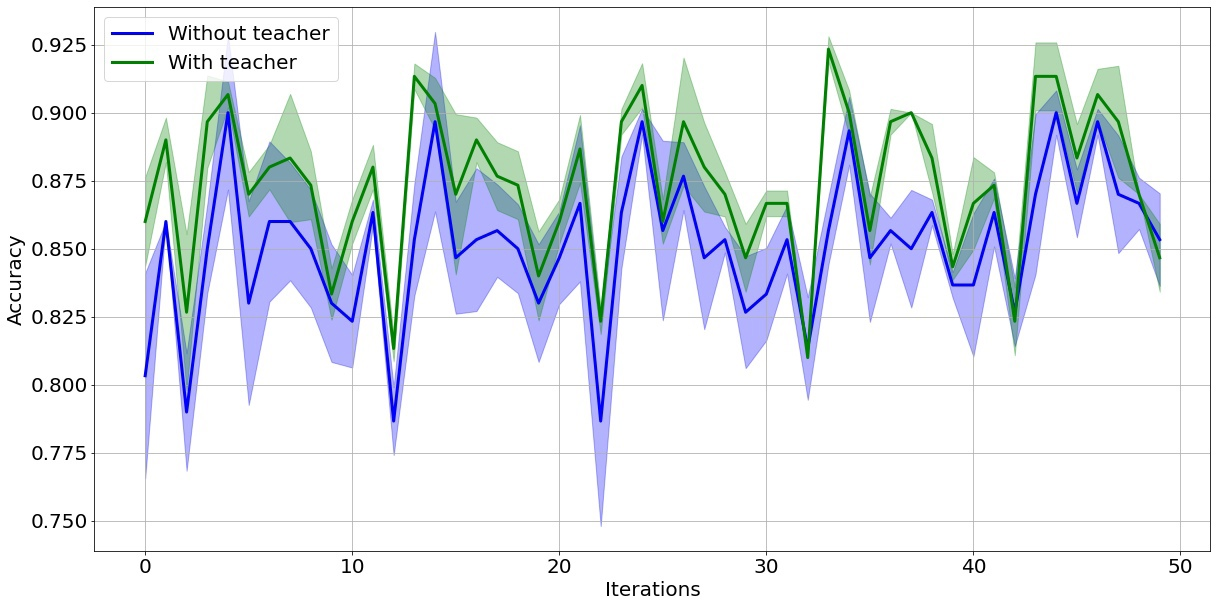
\includegraphics[width=0.5\textwidth]{results/acc_big}}
\subfloat[]
{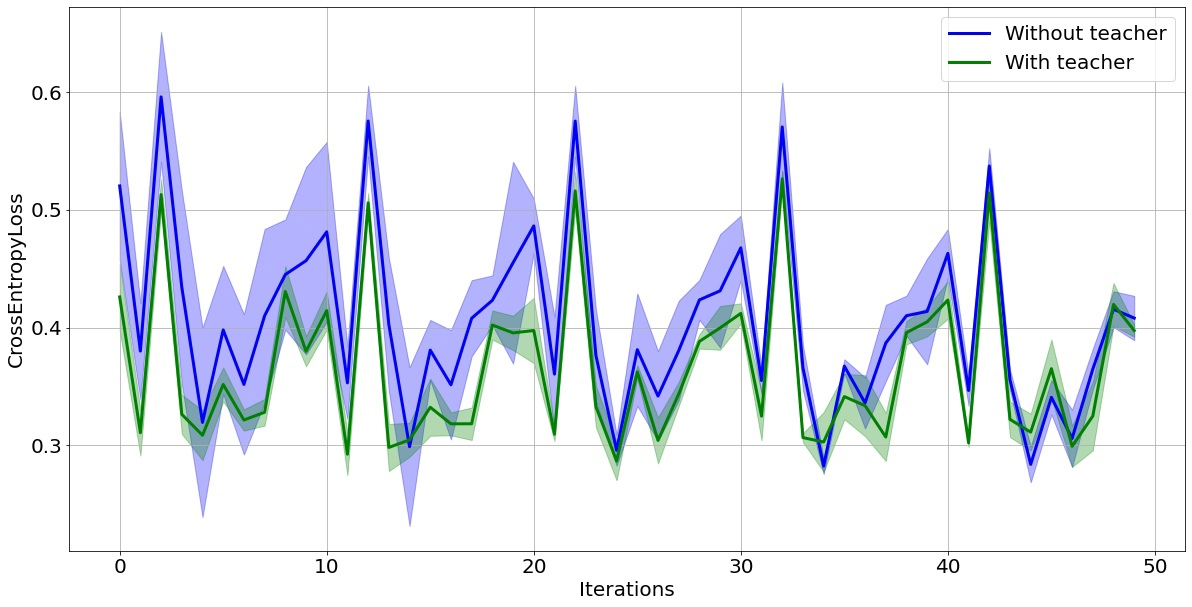
\includegraphics[width=0.5\textwidth]{results/loss_big}}\\
\caption{Качество аппроксимации на тестовой выборке a) accuracy; b) CrossEntropyLoss между истинными и предсказанными учеником метками}
\end{figure}

\newpage
\textbf{Обучение на малоресурсном домене}
На рис.1а показан график зависимости метрики accuracy на тестовой выборке между истинными метками объектов и вероятностями, предсказанными моделью ученика.\\
На рис.1б показан график зависимости кросс-энтропии на тестовой выборке между истинными метками объектов и вероятностями, предсказанными моделью ученика.\\
На графиках видно, что модель, использующая метки учителя, показывает лучшее значение accuracy, при этом наблюдается незначительное повышение ошибки.
\begin{figure}[h!t]\center
\subfloat[]
{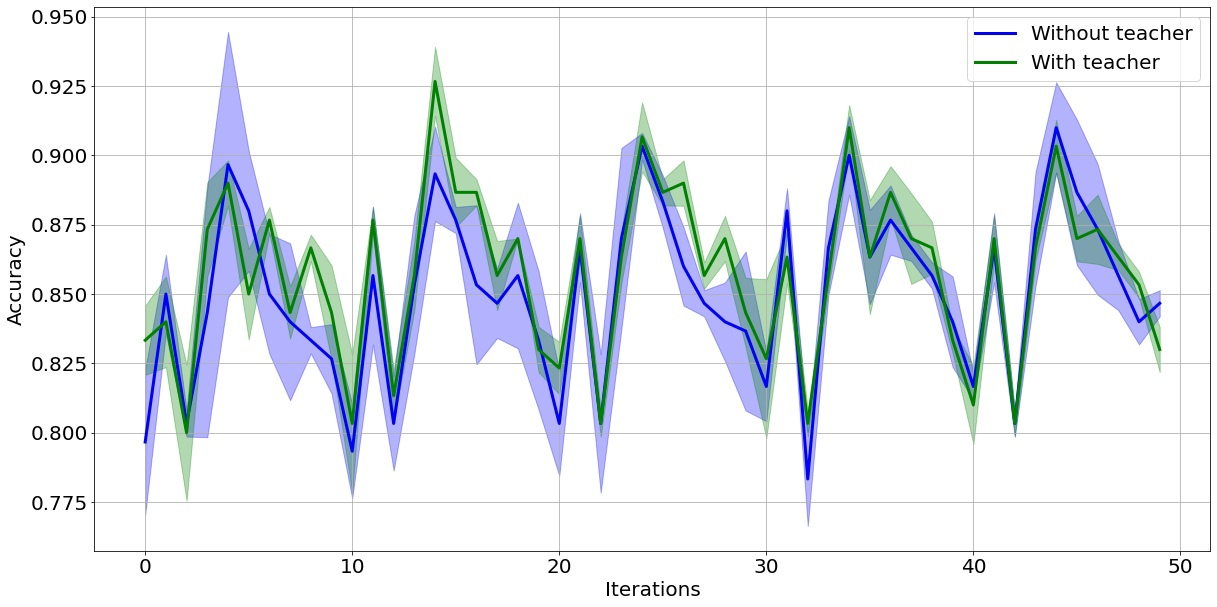
\includegraphics[width=0.5\textwidth]{results/acc_small}}
\subfloat[]
{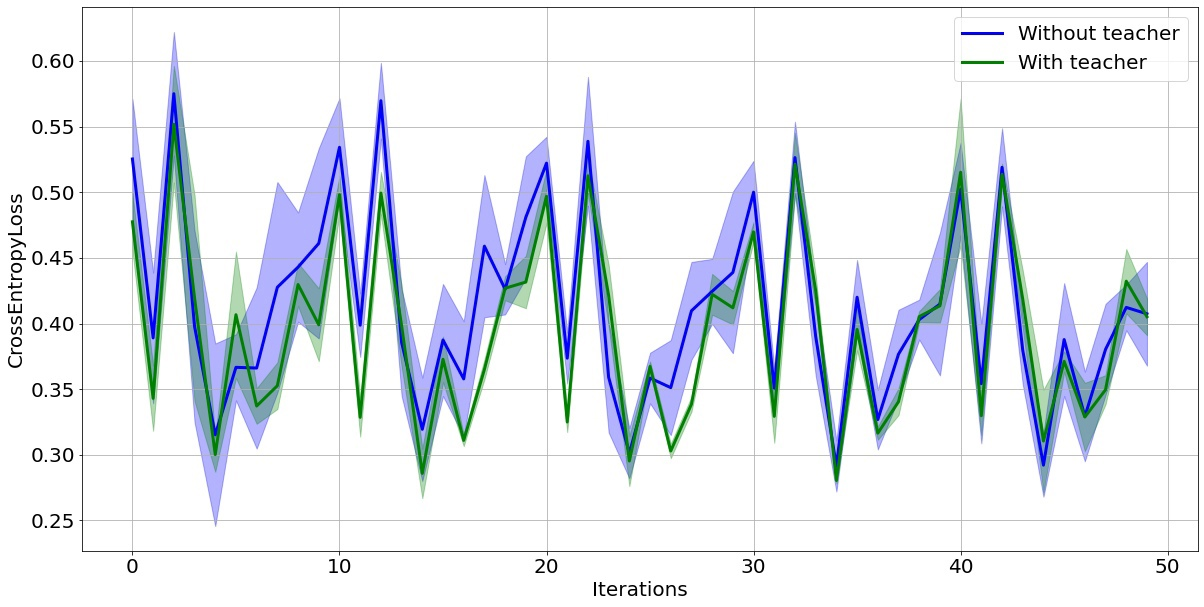
\includegraphics[width=0.5\textwidth]{results/loss_small}}\\
\caption{Качество аппроксимации на тестовой выборке a) accuracy; b) CrossEntropyLoss между истинными и предсказанными учеником метками}
\end{figure}
